\label{app:prescribing-safety-indicators}
This appendix provides methodological detail on prescribing safety indicator implementation (\ref{app:prescribing-safety-indicators-subsection}-\ref{app:prescribing-safety-indicators-prevalence}) and supplementary analyses of System performance against these indicators (\ref{app:prescribing-safety-indicators-clinician-indicator-agreement}-\ref{app:prescribing-safety-indicators-performance-by-type}).
\subsection{Prescribing Safety Indicators}
    \label{app:prescribing-safety-indicators-subsection}
    The PINCER (Pharmacist-Led Information Technology Intervention for Medication Errors) methodology provides evidence-based prescribing safety indicators useful for automated extraction from GP electronic health records \cite{Avery2012}. These were later expanded to a set of 56 prescribing safety indicators for GPs \cite{Spencere181}. The indicators identify specific medications, diagnoses, and monitoring gaps that represent prescribing errors with clear contraindications. A set of 10 prescribing safety indicators were selected to identify complex patients for inclusion in the test set and to enable direct evaluation against distinct criteria.

    The indicators first needed to be translated from English descriptions into executable SQL queries that would run on our EHR export. Each criterion required identifying dozens of relevant SNOMED CT codes, implementing temporal logic for medication durations and monitoring windows, and ensuring the query logic accurately reflects clinical intent. We developed a novel semi-automated approach using Claude Code, an agentic AI coding assistant, and a Model Context Protocol (MCP) server providing access to the SNOMED CT database. The code for this is open sourced.
    
    
    \begin{table}[h]
        

        \centering
        \begin{tabular}{@{}clp{10cm}@{}}
        \toprule
        \textbf{Step} & \textbf{Component} & \textbf{Description} \\
        \midrule
        1 & Input & English description of indicator provided to Claude Code \\
        2 & Code lookup & MCP server provides real-time SNOMED CT code lookups, identifying relevant codes and their parent/children \\
        3 & Query generation & Claude Code generates SQL filter queries implementing the criterion's logic \\
        4 & Validation & Generated queries tested against patient database to verify clinically sensible matches \\
        \bottomrule
        \end{tabular}
        \caption{Workflow for translating PINCER prescribing safety indicators into executable SQL queries using Claude Code and an MCP server for real-time SNOMED CT lookups, followed by database validation.}
    \label{tab:queries}
    \end{table}

    Queries were generated using the workflow detailed in Table~\ref{tab:queries}. This approach enabled rapid iteration and systematic exploration of SNOMED code hierarchies that would have been prohibitively time-consuming manually. For example, identifying all UK dm+d codes for ``non-selective NSAIDs'' required enumerating dozens of specific medication formulations, which the MCP-enabled system could retrieve. This methodology was particularly effective as our evaluation objective required high confidence positive cases rather than comprehensive capture of all potential instances.

    Two additional filters (16 and 43) were excluded due to implementation errors identified during validation. Filters identified patients meeting the error criteria continuously for at least 14 days after January 1, 2020, to exclude brief periods that could be the result of data errors and not clinically relevant.

\subsection{Prescribing Safety Indicators Prevalence}
\label{app:prescribing-safety-indicators-prevalence}

    Table \ref{tab:filter_distribution} shows the 8 validated filters and their prevalence in the 200,000-patient test population. 

    \begin{table}[ht]
    \centering
    \begin{tabular}{@{}lrrr@{}}
    \toprule
    \textbf{Prescribing Safety Indicator} & \textbf{\begin{tabular}[c]{@{}r@{}}Matched\\patients\end{tabular}} & \textbf{\begin{tabular}[c]{@{}r@{}}Prevalence\\per million\end{tabular}} & \textbf{\begin{tabular}[c]{@{}r@{}}\% of time\\matching\end{tabular}} \\
    \midrule
    Filter 05: Diltiazem/verapamil + HF & 17 & 8 & 9.2\\
    Filter 06: Beta-blocker + asthma & 2279 & 647 & 5.5\\
    Filter 10: Antipsychotic + dementia & 273 &  176 & 12.8\\
    Filter 23: CHC + obesity (BMI $\geq$40) & 34 & 15 & 8.6\\
    Filter 26: Methotrexate without folic acid & 493 &  199 & 7.1\\
    Filter 28: NSAID + peptic ulcer & 97 & 10 & 1.8\\
    Filter 33: Warfarin + antibiotic & 337 & 49 & 1.2\\
    Filter 55: Methotrexate without LFT & 454 & 249 & 9.6\\
    \bottomrule
    \end{tabular}
    \caption{Distribution of 8 validated prescribing safety indicators in the source population of 200,000 patients. Matched patients are individuals who matched the filter at least once from 2020 for $\geq$14 days. The prevalence reflects the expected number per million individuals flagged at any given moment (point prevalence), which is lower than cumulative matched patients because individuals were not flagged continuously from 2020. The percentage of time matching indicates, for patients who matched a filter at any point, the proportion of time that filter flagged them since 2020.}
    \label{tab:filter_distribution}
    \end{table}

    \noindent
    A total of 3,984 unique patients in the 200,000-patient test set matched at least one of the 8 indicators during the evaluation period, representing a combined point prevalence of approximately 0.14\%. Individual filter prevalence varied substantially, from 8 patients per million for Filter 5 (diltiazem/verapamil + heart failure) to 647 per million for Filter 6 (beta blocker + asthma). Among patients who matched a filter at any point since 2020, the proportion of time continuously meeting criteria ranged from 1.2\% (Filter 33: Warfarin + antibiotic) to 12.8\% (Filter 10: antipsychotic + dementia), reflecting both the transient nature of some prescribing errors and the chronic persistence of others.


\subsection{Clinician-indicator Agreement}
\label{app:prescribing-safety-indicators-clinician-indicator-agreement}

    Among the 73 indicator-positive cases included in the analysis (after excluding filters 16 and 43), the clinician agreed with the indicator classification in 51 cases (69.9\%). In 22 cases (30.1\%), the clinician disagreed that intervention was warranted for the identified indicator. Notably, among these disagreements, the clinician identified alternative clinical issues in 20 cases (90.9\% of all disagreed cases). Agreement varied substantially by indicator type as shown in Table \ref{tab:clinician_indicator_agreement}.

    \begin{table}[ht]
        \centering
        \begin{tabular}{@{}lrrr@{}}
        \toprule
        \textbf{Prescribing Safety Indicator} & \textbf{\begin{tabular}[c]{@{}r@{}}Cases\\reviewed\end{tabular}} & \textbf{\begin{tabular}[c]{@{}r@{}}Clinician\\agreed\end{tabular}} & \textbf{\begin{tabular}[c]{@{}r@{}}Agreement\\\%\end{tabular}} \\
        \midrule
        Overall & 73 & 51 & 69.9 \\
        \midrule
        Filter 05: Diltiazem/verapamil + HF & 6 & 6 & 100.0 \\
        Filter 28: NSAID + peptic ulcer & 9 & 9 & 100.0 \\
        Filter 26: Methotrexate without folic acid & 9 & 7 & 77.8 \\
        Filter 33: Warfarin + antibiotic & 10 & 7 & 70.0 \\
        Filter 23: CHC + obesity (BMI $\geq$40) & 9 & 6 & 66.7 \\
        Filter 06: Beta-blocker + asthma & 10 & 6 & 60.0 \\
        Filter 10: Antipsychotic + dementia & 9 & 5 & 55.6 \\
        Filter 55: Methotrexate without LFT & 10 & 5 & 50.0 \\
        \bottomrule
        \end{tabular}
        \caption{Clinician agreement with prescribing safety indicators. Among 73 indicator-positive cases reviewed, the clinician agreed that intervention was warranted in 51 cases (69.9\%). Agreement varied by indicator type, with absolute contraindications (Filters 5, 28) achieving 100\% agreement and monitoring-based indicators showing lower agreement.}
        \label{tab:clinician_indicator_agreement}
    \end{table}

    The 30.1\% disagreement rate demonstrates that deterministic criteria do not fully capture the contextual clinical judgment required for medication safety assessment. Even expert-validated tools require contextual judgment for application. However, the high rate of alternative issues identified in disagreed cases (90.9\%) indicates that indicator-positive patients represent genuinely complex cases requiring review, even when the specific indicator flag may not warrant intervention.

\subsection{Hierarchical Performance Against Prescribing Safety Indicators}

    \begin{table}[htbp]
        \centering

        \begin{tabular}{@{}llrr@{}}
        \toprule
        \textbf{Case Type} & \textbf{Evaluation Level} & \textbf{Number of patients} & \textbf{Rate} \\
        \midrule
        \multicolumn{4}{l}{\textbf{Validated Prescribing Safety Indicator (n=52)}} \\
        \midrule
        & \textit{Level 1: Issue Identification} & & \\
        & \quad Issue identified & 52 & 100.0\% \\
        & \quad Issue not identified & 0 & 0.0\% \\
        \cmidrule(lr){2-4}
        & \textit{Level 2: Issue Correctness} & & \\
        & \quad Correct issue & 43 & 82.7\% \\
        & \quad Incorrect issue & 9 & 17.3\% \\
        \cmidrule(lr){2-4}
        & \textit{Level 3: Intervention Appropriateness} & & \\
        & \quad Correct intervention & 40 & 76.9\% \\
        & \quad Incorrect intervention & 3 & 5.8\% \\
        & \quad Did not reach Level 3 & 9 & 17.3\% \\
        \bottomrule
        \end{tabular}
        \caption{Performance Against Prescribing Safety Indicators. Analysis restricted to 52 cases where clinician validated that the indicator flag correctly identified an issue requiring intervention (from 73 total indicator-positive cases after excluding filters 16 and 43).}
        \label{tab:pincer_performance}
    \end{table}

    Against clinician-validated indicator cases (Table~\ref{tab:pincer_performance}), the System achieved perfect Level 1 sensitivity, identifying all 52 cases requiring intervention (100\%). At Level 2, the system correctly identified the specific indicator in 43 cases (82.7\%), with 9 cases where the System flagged an issue but did not identify the indicator was present. At Level 3, among the 43 correctly identified issues, appropriate interventions were proposed in 40 cases (76.9\% of all positive cases, 93.0\% conditional on Level 2 success).

\subsection{Performance by Filter Type}
    \label{app:prescribing-safety-indicators-performance-by-type}

    Performance varied substantially across the 8 validated indicators as shown in Figure~\ref{fig:performance-by-filter}. Mean clinician scores ranged from 0.50 (Filter 23: combined hormonal contraception with obesity, BMI $\geq$ 40) to 0.80 (Filter 28: NSAID + peptic ulcer), with most filters clustering between 0.60 and 0.80. 

    Filter 28 (NSAID + peptic ulcer) achieved the highest mean score of 0.80 with lower performance from Filter 23 (0.50), Filter 6 (beta-blocker + asthma, 0.60), and Filter 55 (methotrexate without LFT monitoring, 0.59).

    Interpretation is complicated by the small number of clinician-validated cases per filter (range: 6-9 patients per filter after clinician disagreement exclusions), leading to wide confidence intervals that limit robust conclusions about filter-specific performance patterns.

    \begin{figure}[ht]
        \centering
        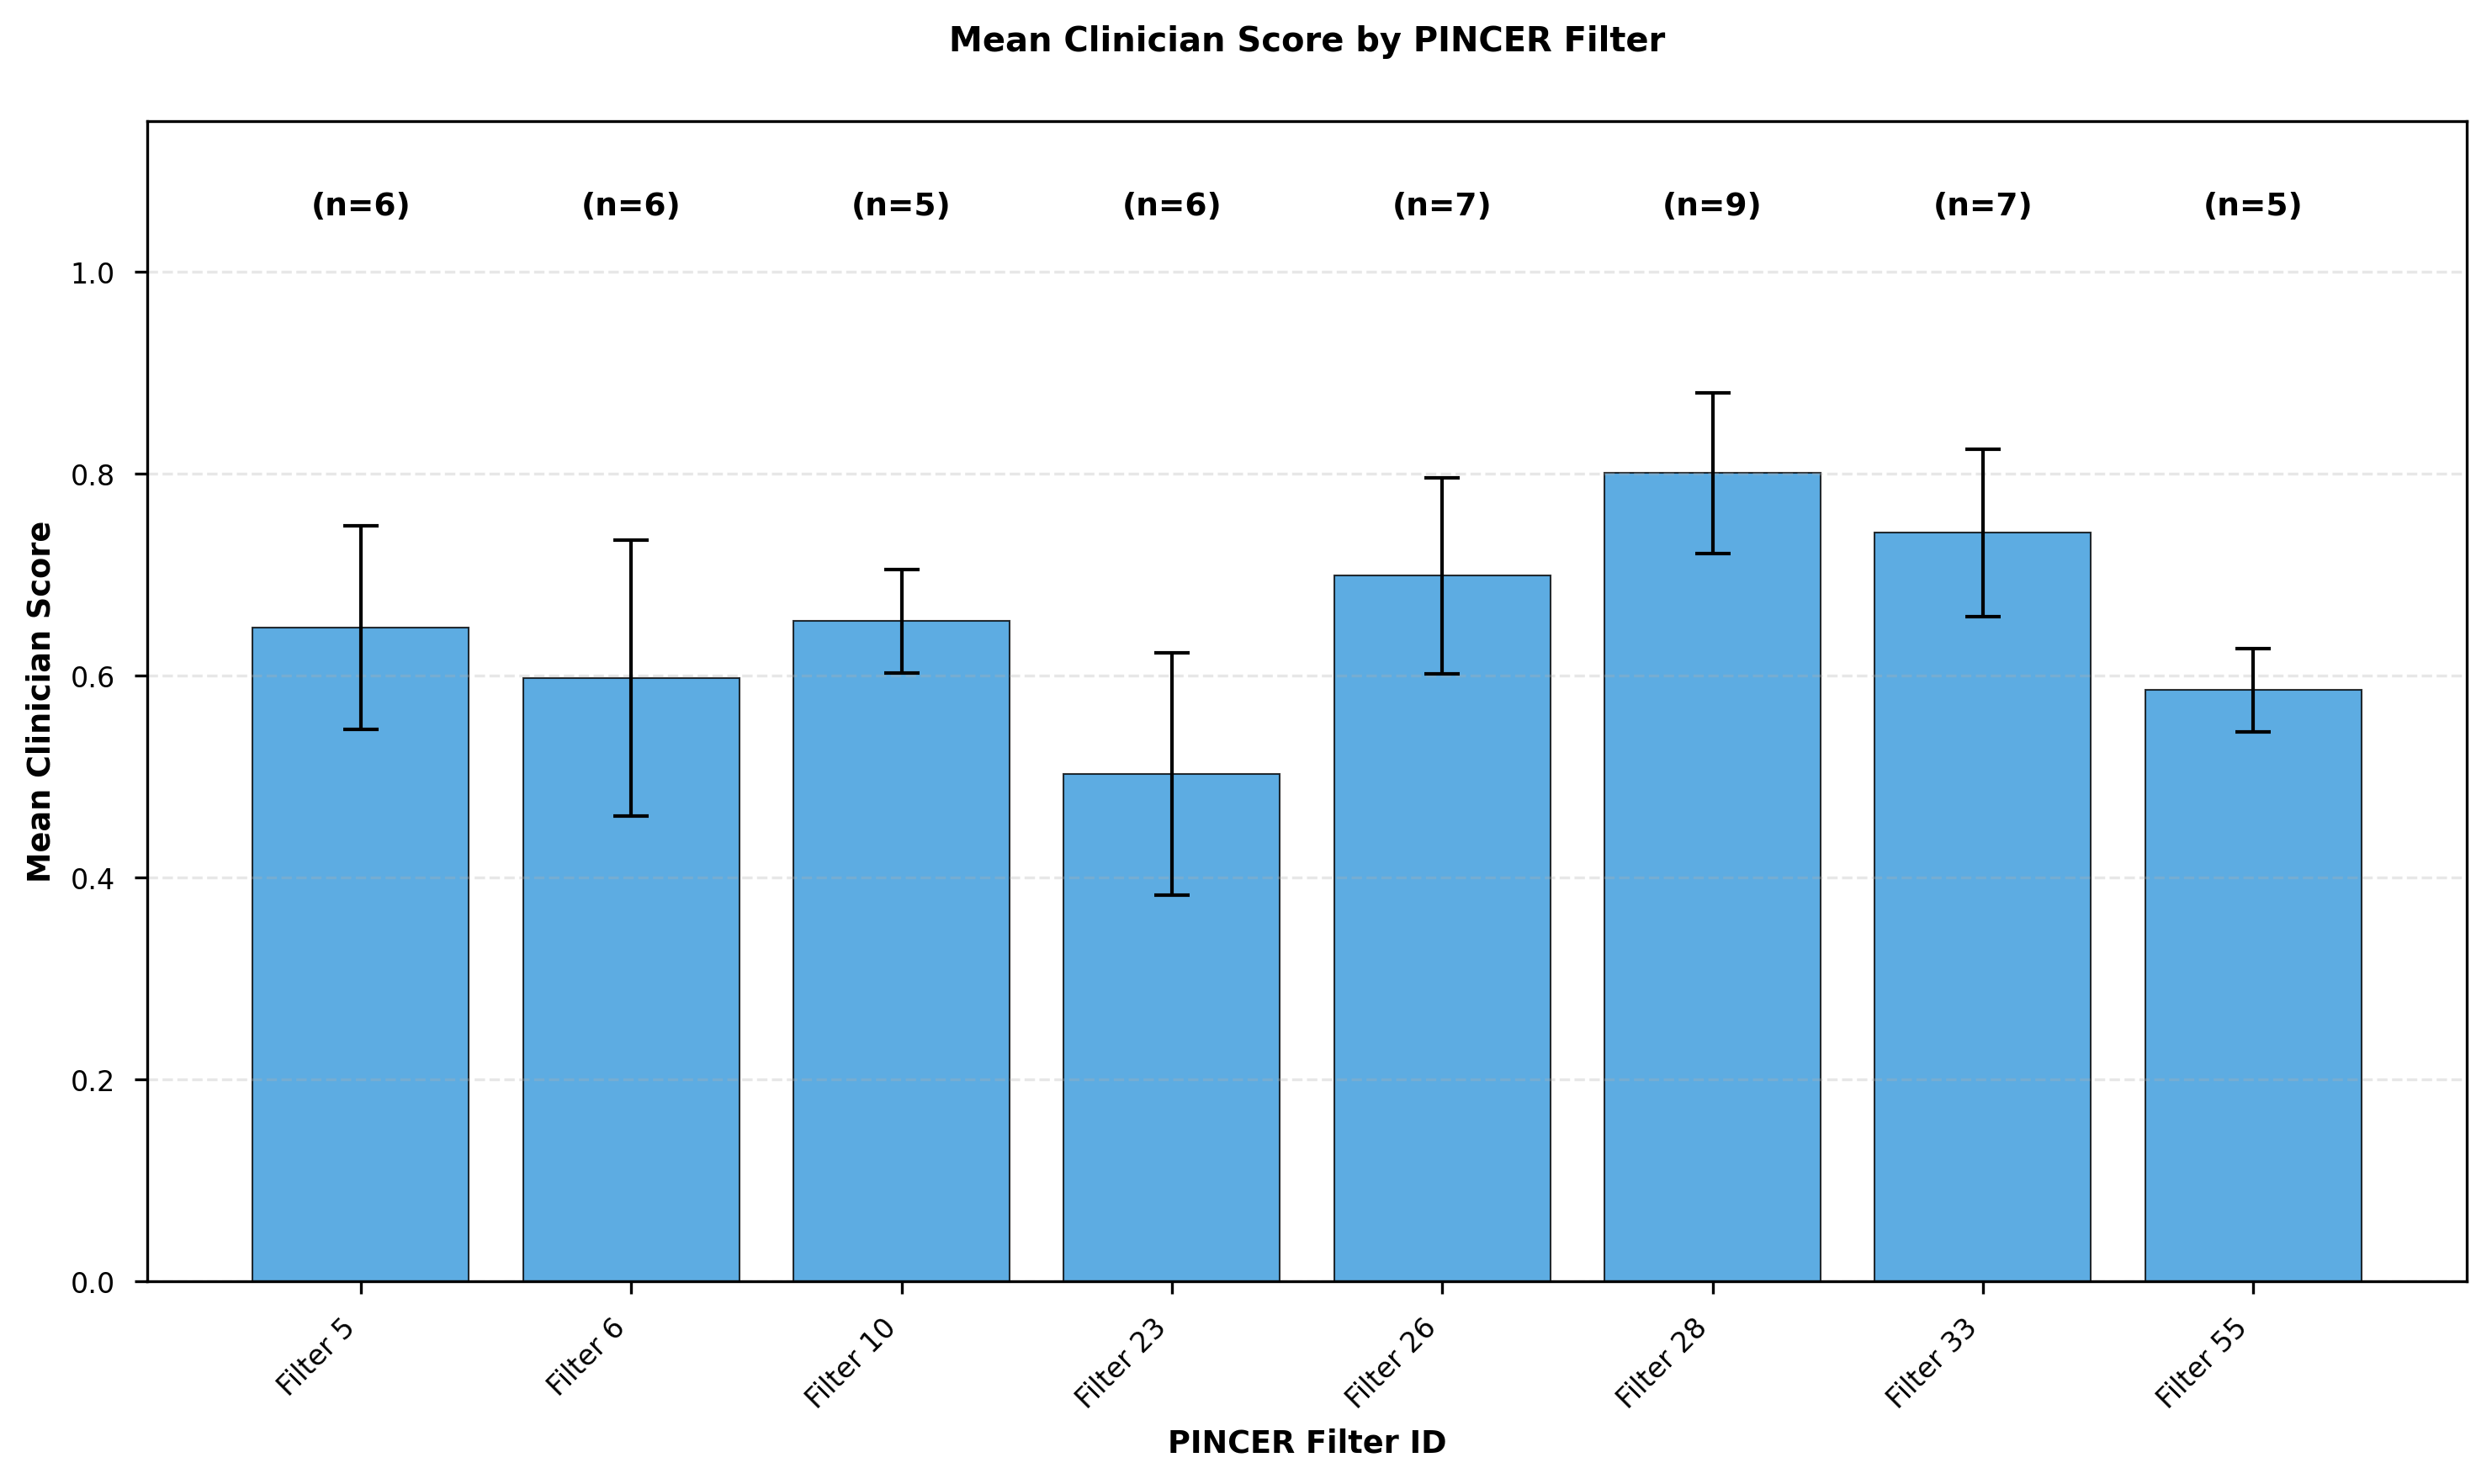
\includegraphics[width=0.8\textwidth]{figures/performance_by_filter_clinician.png}
        \caption{the System's performance by indicator. Mean clinician scores shown with standard error bars. Sample sizes per filter range from 6-9 patients (only cases where clinician validated intervention was needed). Eight filters shown after excluding filters 16 and 43 due to implementation errors.}
        \label{fig:performance-by-filter}
    \end{figure}